\documentclass{article}

\usepackage{lmodern}
\usepackage[T1]{fontenc}
\usepackage[spanish,activeacute]{babel}
\usepackage[utf8]{inputenc}
\usepackage{hyperref}
\usepackage[left=1.5cm,top=1.5cm,right=2cm,bottom=1.5cm]{geometry}
\usepackage{graphicx} 
\usepackage{listings}

\title{Tarea 3: No somos nada, hola Internet}
\author{Esteban Hernández\\estebanhernandezv@alumnos.usm.cl\\201173559-5.\and Cristian Yáñez\\cristian.yanez@alumnos.usm.cl\\201173504-8 \and \\Campus San Joaquín }

\begin{document}

\begin{titlepage}
\maketitle
\end{titlepage}

\section{} 
Utilizando la herramienta Open Visual Traceroute, observamos el recorrido que hicieron las solicitudes para cada página web. Los recorridos son los siguientes:

\subsection{http://moodle.inf.utfsm.cl/}
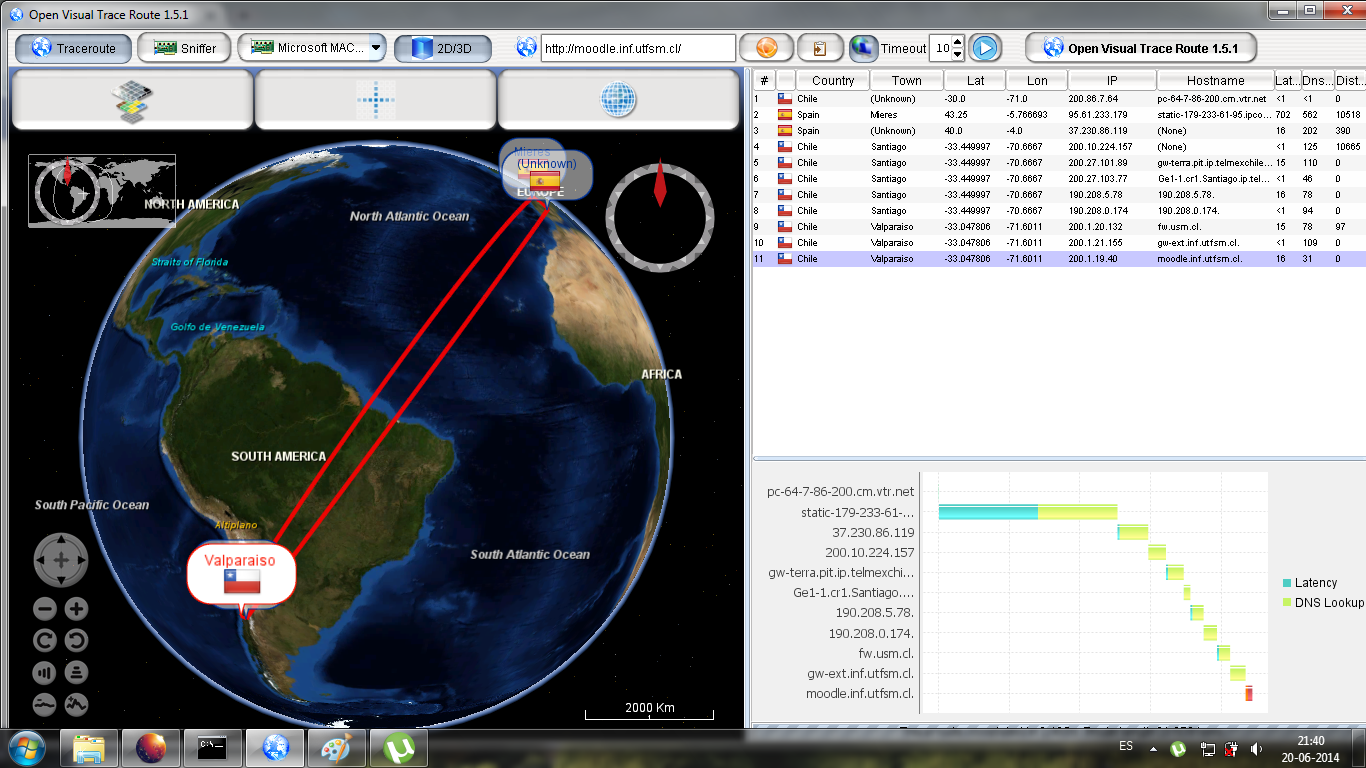
\includegraphics[scale=0.52]{Img/moodle.png} 
Para Moodle, se puede observar de que se realizaron muchos saltos (11 en este caso), y aunque la mayoría de estos se hacen en Territorio Nacional (Santiago y Valparaíso), un par de éstos son hacia España. Esto se produjo debido a que el primer router por el que pasó la información decidió que la ruta óptima era hacia España y de vuelta, decisión que seguramente tomó debido a que las conexiones en Chile al momento de realizar el test estaban con mucho tráfico.

\subsection{http://google.cl/}
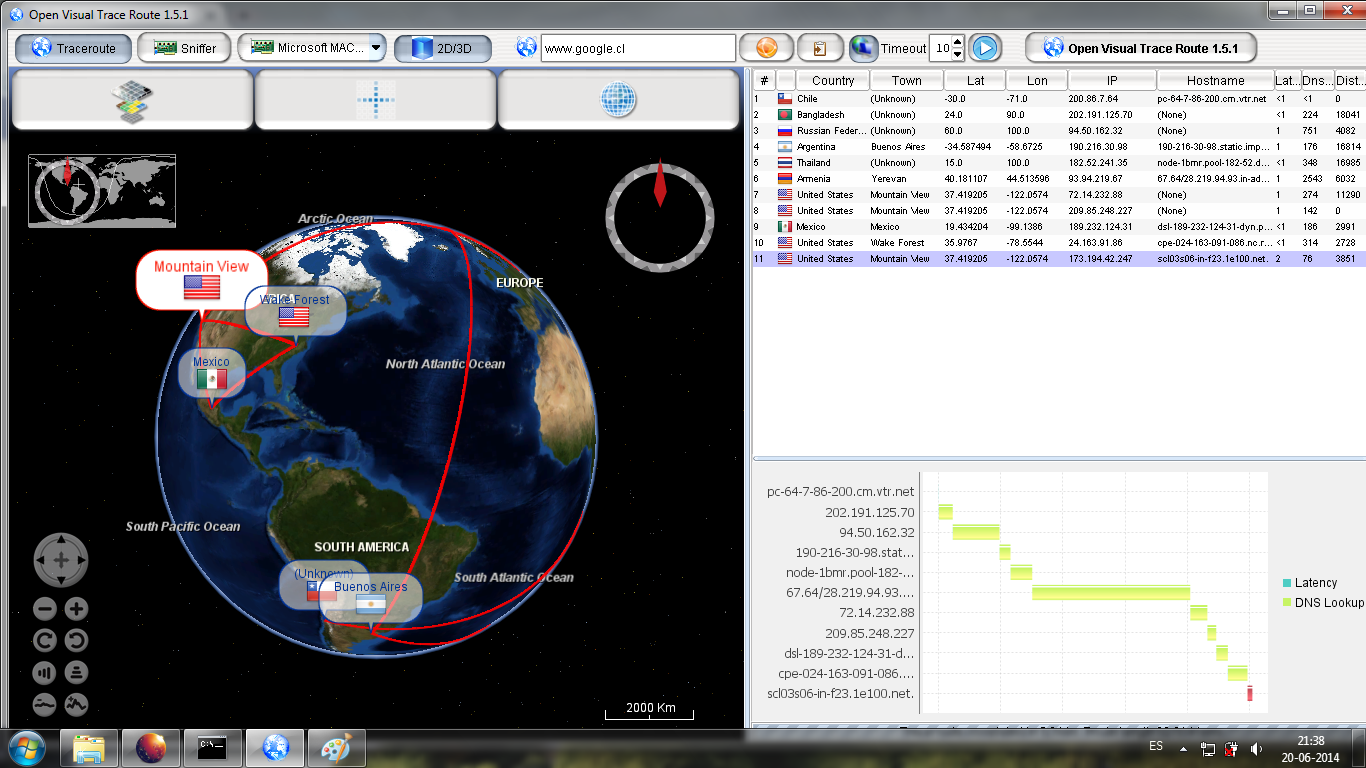
\includegraphics[scale=0.52]{Img/google.png} 
En el caso de Google, se observa el paso de la información por una gran cantidad de países (Chile, Bangladesh, Rusia, Argentina, Tailandia, Armenia, México y EE.UU). Esta gran cantidad se debe al despliegue que tiene la empresa Google en el mundo, y a todos los lugares en los que se encuentra.\\ Nuevamente, el gran viaje de la información se debe probablemente a la saturación en las redes Nacionales y/o Latino-Americanas, lo que no permitió un traspasó mas directo hacia la ciudad de Mountain View.


\subsection{http://cime.cl/}
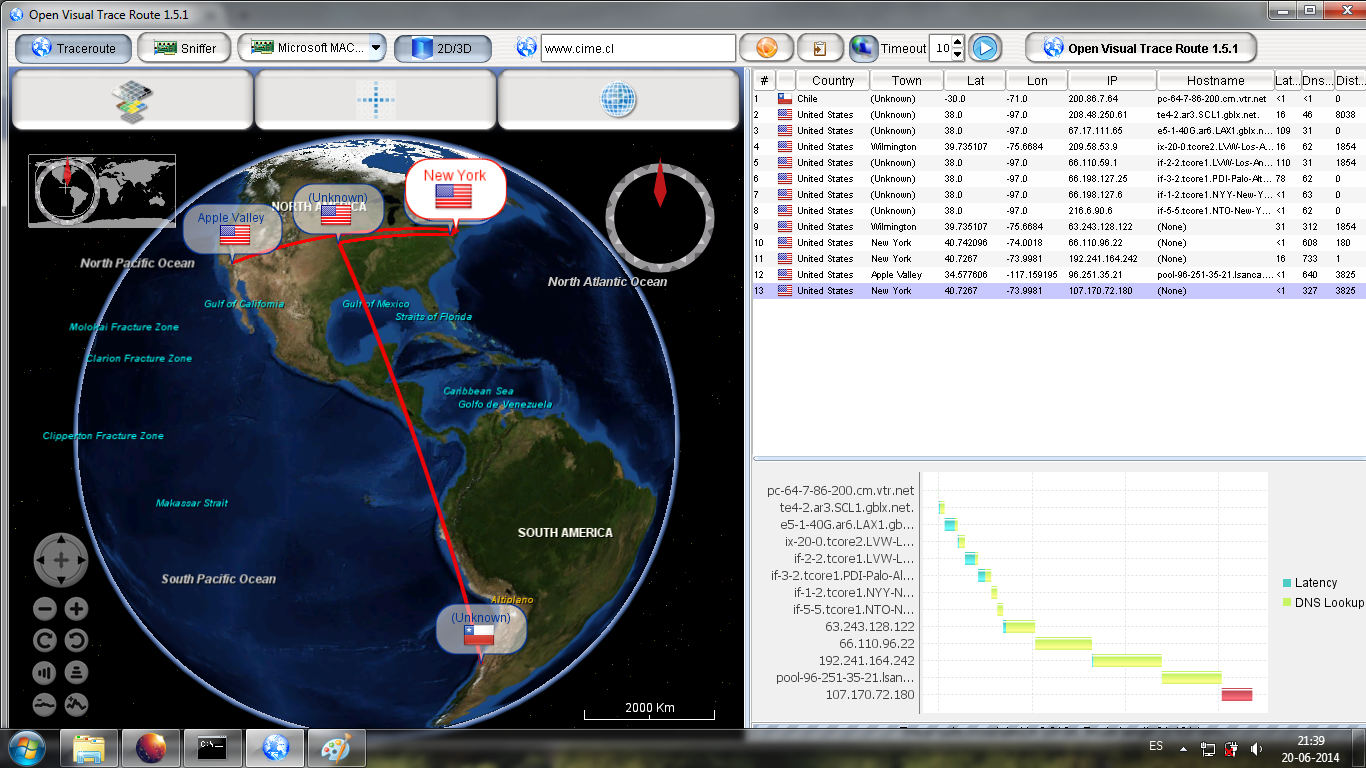
\includegraphics[scale=0.52]{Img/cime.png} 
Al observar este caso, lo primero que destaca es que aunque existan gran cantidad de saltos (13), 12 de ellos son en EE.UU, donde la información va pasando por distintas ciudades hasta llegar al servidor en donde se aloja la página, ubicado en Nueva York. Esta vez los routers Norteamericanos fueron los encargados de observar sus tablas de enrutamiento y elegir la mejor ruta.


\subsection{http://wikipedia.com/}
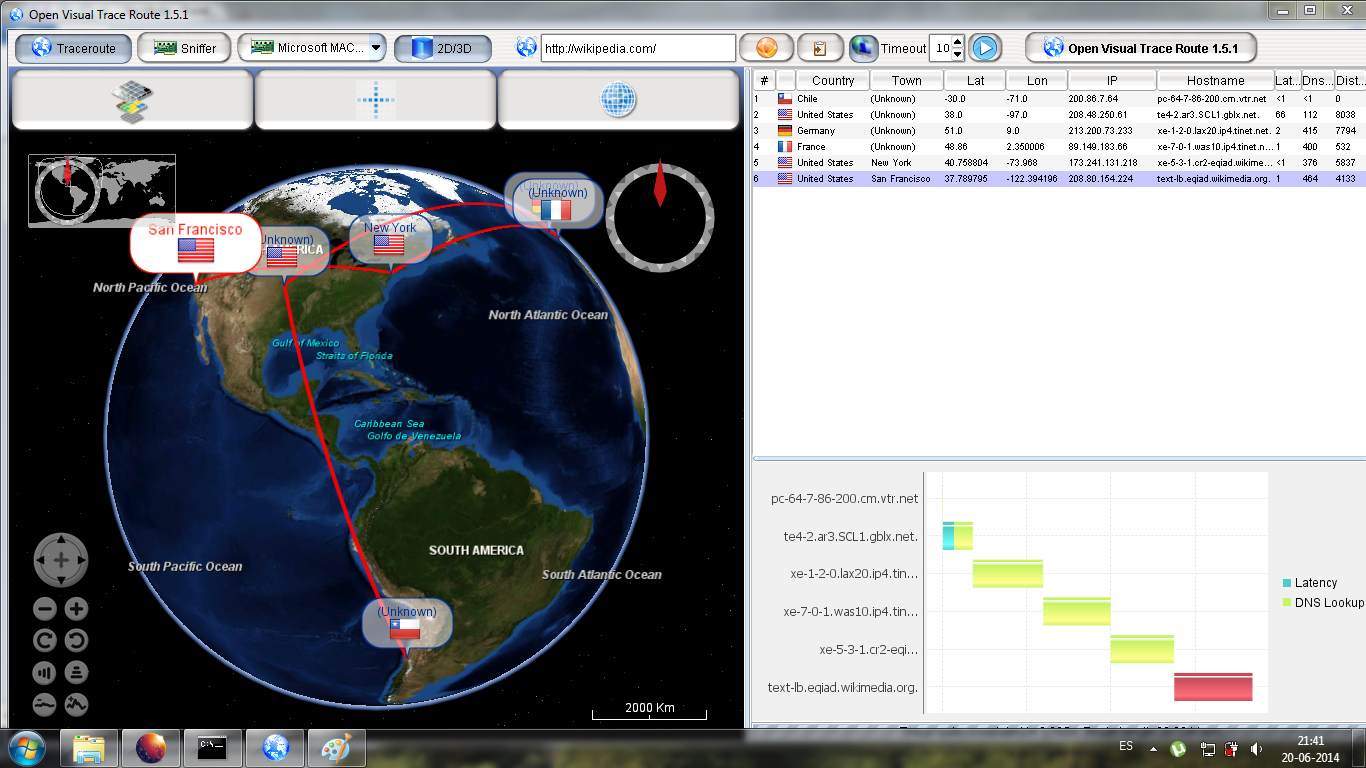
\includegraphics[scale=0.52]{Img/wikipedia.png} 
Al contrario que en los casos anteriores, al solicitar la página de Wikipedia esta solicitud pasa por una menor cantidad de saltos que las demás páginas (6 exactamente), pero aún así debió recorrer 4 países distintos (Chile, Alemania, Francia y EE.UU) para llegar finalmente a San Francisco, EE.UU.


\subsection{http://www.chile.embassy.gov.au/}
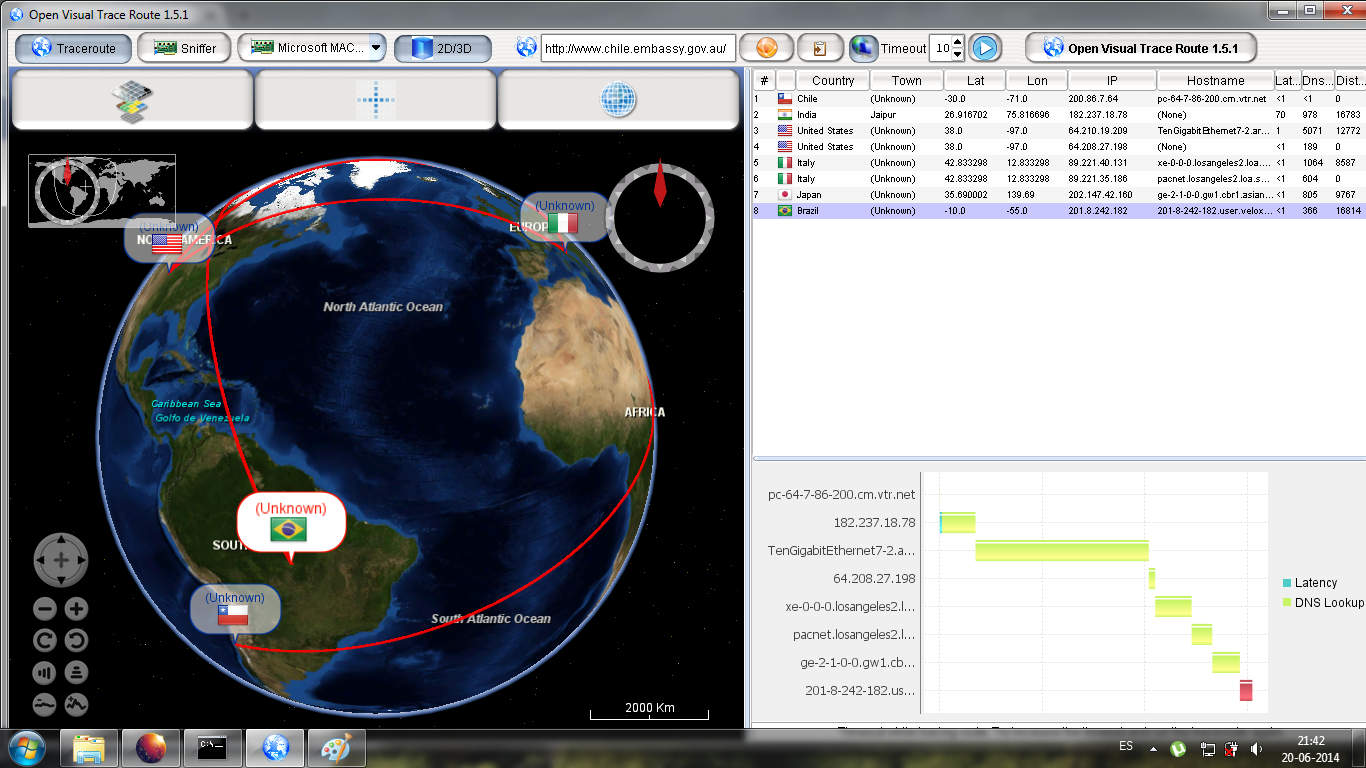
\includegraphics[scale=0.52]{Img/embajada.png} 
El caso mas extraño es éste, dado que aunque se trata de la página de la embajada de Chile en Australia, las solicitudes jamas pasan por estos países (exceptuando al inicio). Otra observación es la gran distancia que recorre la información, la que como se ve en la imagen, recorre India, EE.UU, Italia, Japón y Brasil.


\subsection{¿Y como viaja la información?}

Para la conexión entre continentes, existen cables submarinos hechos de fibra óptica, de 7 cm aprox. de espesor, los cuales recorren miles de kilómetros para poder intercambiar información (en forma de paquetes) entre continentes muy lejanos rápidamente. \cite{CAB} \\ Como señala el artículo, antiguamente estos cables solo eran capaces de conectar dos puntos geográficos, pero actualmente existen \emph{ramificadores} capaces de separar el cable en otros distintos y así alcanzar varios lugares.\\
Otro punto importante, dado la longitud de estos cables, es la posible atenuación o pérdida de la señal. Este fenómeno es mitigado con aparatos llamados \emph{repetidores}, que son puestos aproximadamente cada 100kms y que son capaces de retransmitir la señal que reciben a una mayor potencia, evitando así la atenuación de la señal.\\
Uno de los riesgos que posee el tener cables submarinos es la posibilidad de que sean cortados (ya sea accidental o intencionalmente). En caso de que esto ocurra y se deban reparar, el proceso consiste en cortar y subir un extremo del cable a un barco encargado, y luego de probar su buen funcionamiento hacer lo mismo con el otro extremo. Al final de probar el correcto funcionamiento en ambos extremos se unen y se vuelven a hundir (para mayor detalle consultar \cite{REP}).\\
Para tener una idea de la cantidad y alcance de estos cables, se adjunta un mapa de todos los cables intercontinentales que existen hoy en día para el transporte de datos en Internet:\cite{MAP} \\\\
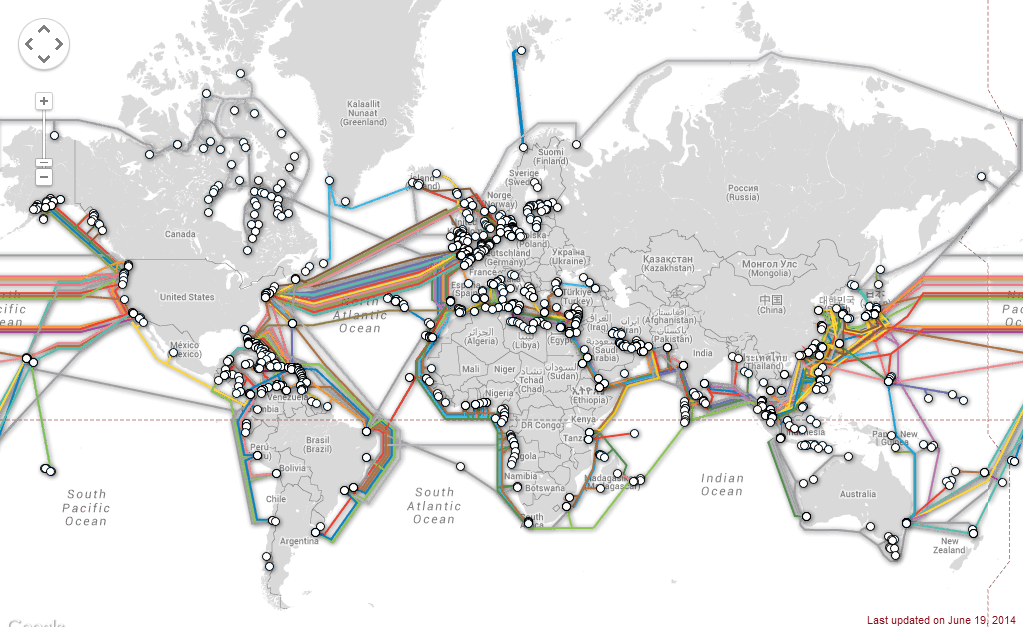
\includegraphics[scale=0.7]{Img/map-world.png} 

\subsection{¿Y en Chile?}

En nuestro país existen 4 cables submarinos encargados de conectarnos con el mundo, los cuales se muestran en las siguientes imagenes:\\
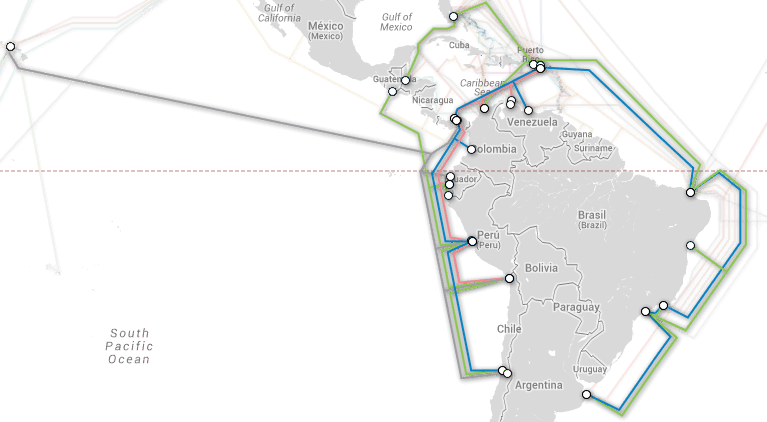
\includegraphics[scale=0.52]{Img/chile2.png}\\
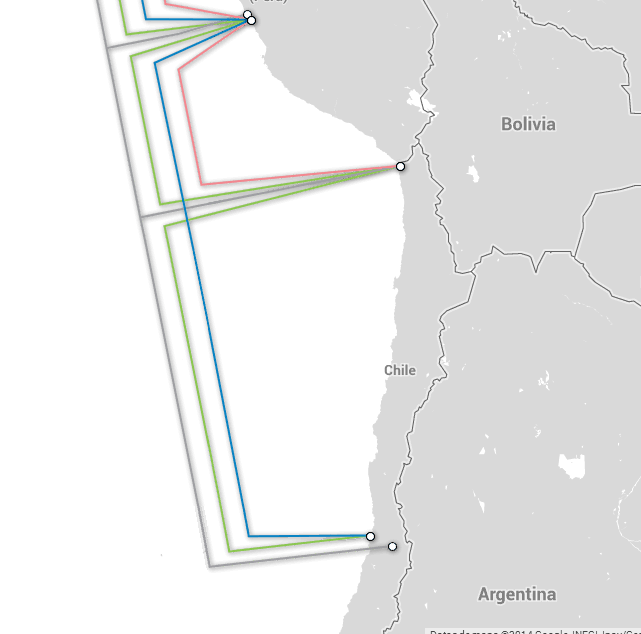
\includegraphics[scale=0.52]{Img/chile.png}\\
Como se observa, los tres "puntos de conexión intercontinental" que posee Chile se ubican en Arica, Valparaíso y Santiago. Los nombres de estos cables son:\\
\begin{itemize}
	\item South America Pacific Link (SAPL) (de color morado en la imagen)
	\item South American Crossing (SAC)/Latin American Nautilus (LAN) (de color azul)
	\item Pan American (PAN-AM) (de color rosado)
	\item South America-1 (SAm-1) (de color verde)
\end{itemize}	



\section{}
Se decide tomar la Alternativa 2 y hacer el trabajo paso por paso:
Primero, el paso 1 es llenar las tablas con los enlaces directos que existen en el grafo. Si no existe conexión directa entre dos routers se llena con $\infty$, y en la conexión entre un router y sí mismo se rellena con el valor 0.\\
Después de pasado un tiempo, cada router entrega su Vector Distancia (VD desde ahora) a sus vecinos, lo que se observa en el paso 2.\\
\centerline{\includegraphics[scale=0.6]{Img/paso12.png}}\\
Luego, como cada router recibió los VD de sus vecinos, deben recalcular sus propios VDs utilizando el algoritmo de Bellman-Ford, el cual dice que cada router debe calcular su VD mediante la fórmula $D_{x}(y) = min_{v}[c(x,v) + D_{v}(y)]$, donde $v$ son todos los vecinos del router, e $y$ representa a todos los nodos del grafo. Por ejemplo, para calcular el nuevo VD del router A se aplica $D_{A}(y) = min[c(A,B) + D_{B}(y), c(A,G) + D_{G}(y),c(A,I) + D_{I}(y)]$, donde $y$ se mueve alfabéticamente entre $A y I$.\\
El resultado se observa en el el Paso 3 (los valores que cambian con respecto al Paso 2 se marcan con color naranja), el que luego da pie al Paso 4 (al cambiar los VD, se deben entregar a sus vecinos).\\
\centerline{\includegraphics[scale=0.5]{Img/paso34.png}}\\
El ciclo explicado anteriormente (Algoritmo de B-F y entregar a sus vecinos) se repite nuevamente, generando así los Pasos 5 y 6 (los cambios de valores entre el paso 4 y 5 se marcan con color azul)\\
\centerline{\includegraphics[scale=0.5]{Img/paso56.png}}\\
Finalmente, se realiza un nuevo paso (se calculan los VD con algoritmo de B-F), pero como no existen variaciones en los números, se llega al Paso 7 y final.\\
\centerline{\includegraphics[scale=0.5]{Img/paso7.png}}\\
De la tabla en el paso 7, se concluye que el mejor camino entre el Router A y el router I tiene como valor 10, y por lo tanto, el valor para la solicitud del PC hacia el Servidor tiene un valor de 14, pasando por los routers A, B, E, I (en ese orden).

\section{}
Al momento de cortarse el enlace, automáticamente los VD de los routers H e I guardan este cambio (dejando sus conexiones como $\infty$,).\\
Como sus VD fueron cambiados, deben ser actualizados mediante el algoritmo de B-F (todo cambio se destacó con color amarillo) y luego de esto enviarlos a los demás Routers vecinos. Al recibir los nuevos VD de H e I, estos routers deben calcular sus propios nuevos VD con B-F. Todo lo anterior queda reflejado en los pasos 8 y 9.\\
\centerline{\includegraphics[scale=0.5]{Img/paso89.png}}\\

Después de aplicar B-F en el Paso 9, los routers E y G varian sus VD, por lo que envían los nuevos a sus respectivos vecinos. Finalmente, estos routers calculan sus propios nuevos VD mediante B-F, pero como no hay cambio, se concluye que la tabla del Paso 10 es la final.\\
\centerline{\includegraphics[scale=0.5]{Img/paso10.png}}\\

Se puede concluir ademas, mirando la tabla nueva del paso 10, que el camino escogido como el mas óptimo en la sección anterior para la conexión entre el Pc y el Servidor (A-B-E-I) no se vé cambiada.


\begin{thebibliography}{1}
\bibitem{CAB} \href{http://www.trenditup.com/trenditup/tecnologia/los-cables-submarinos-que-hacen-posible-que-disfrutes-de-internet/}{Los cables submarinos que hacen posible que disfrutes de Internet}
\bibitem{REP} \href{http://blogthinkbig.com/reparacion-cable-submarino/}{¿Cómo se repara un cable submarino de telecomunicaciones?}
\bibitem{MAP} \href{http://www.submarinecablemap.com/#/country/chile}{Submarine Cable Map}

\end{thebibliography}
\end{document}